\section{Experiments}
\begin{figure*}[t]
\subfigure[Results of the restart policy with the initial $threshold=128$.] { \label{fig:a} 
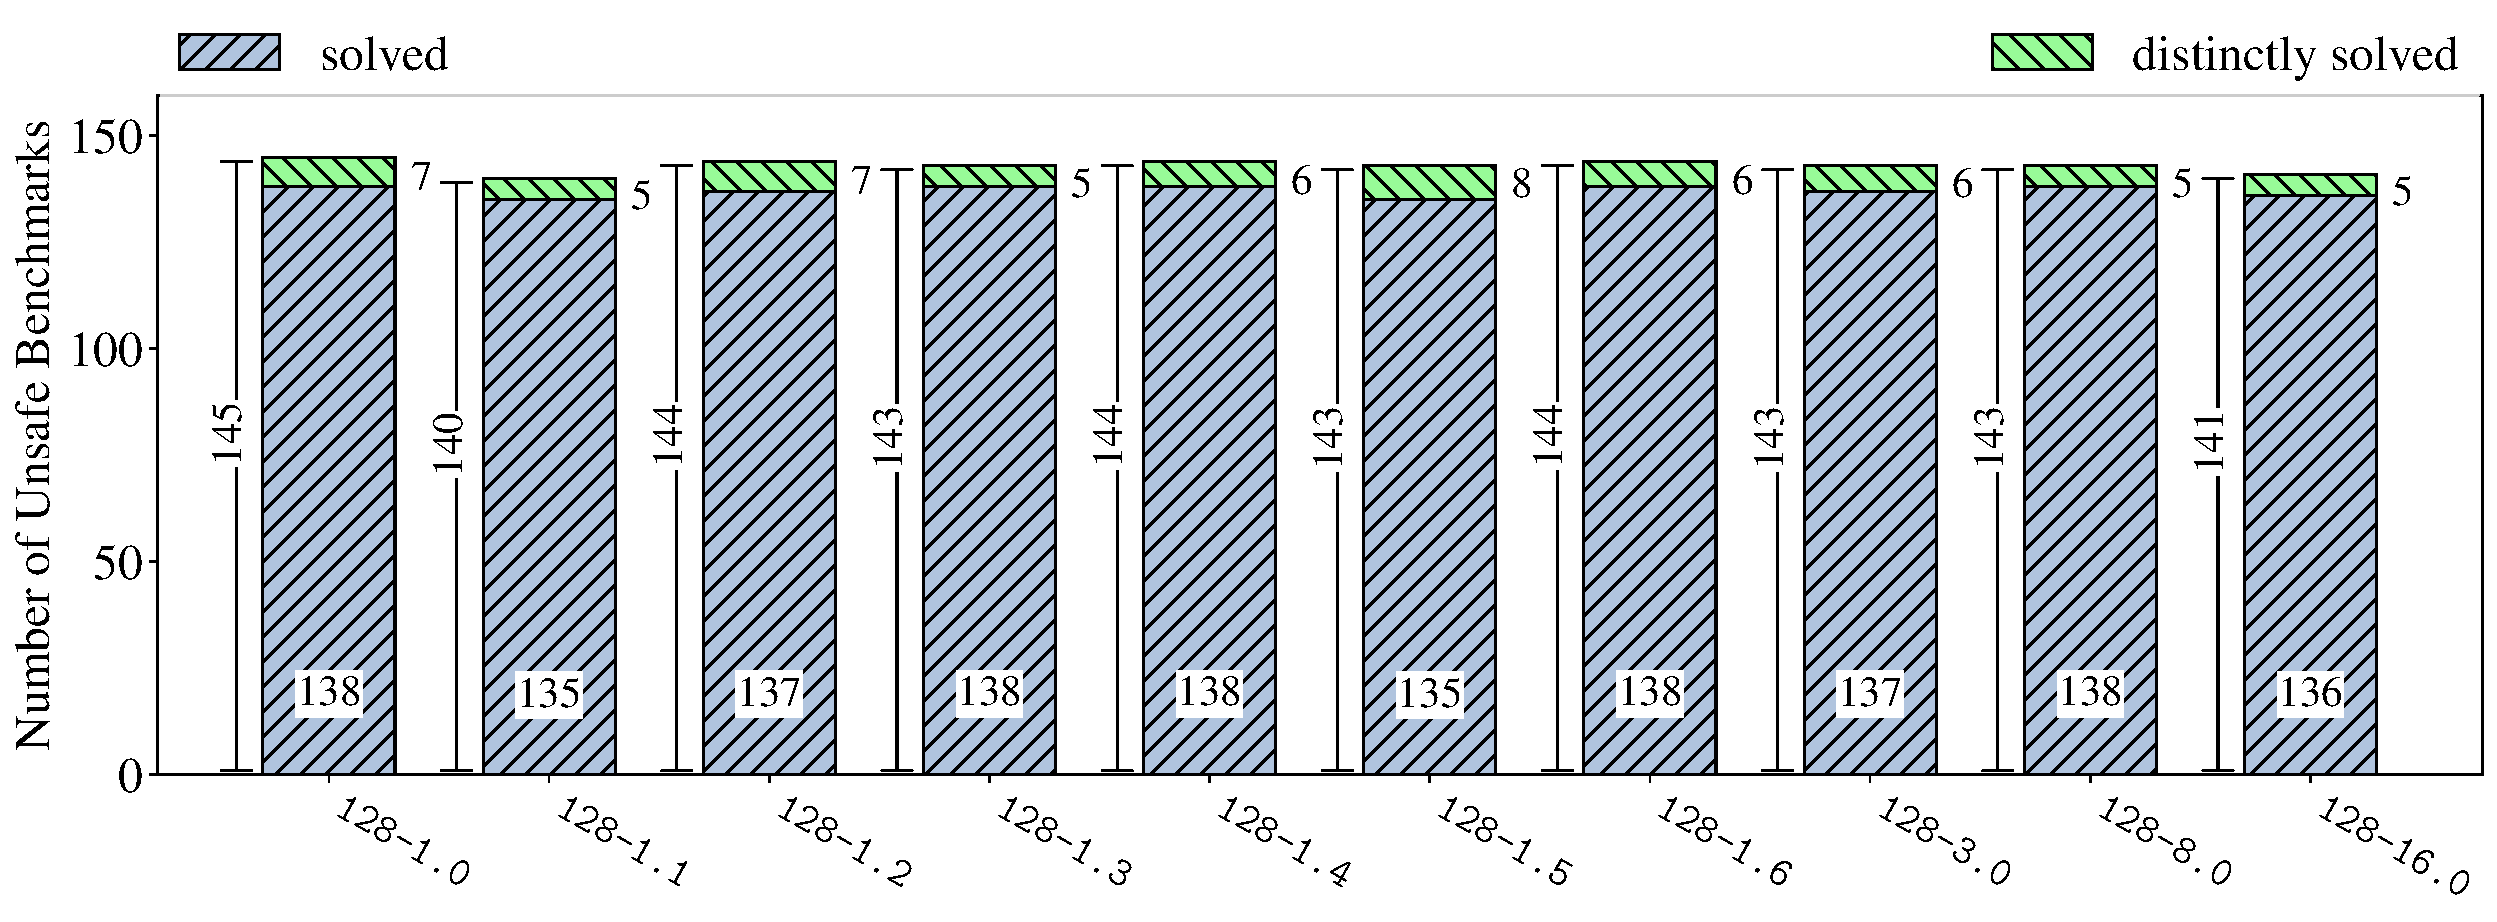
\includegraphics[width=0.98\linewidth]{images/128.pdf} \label{fig:car:128}
}
\subfigure[Results of the restart policy with $gr=1.2$.] { \label{fig:b} 
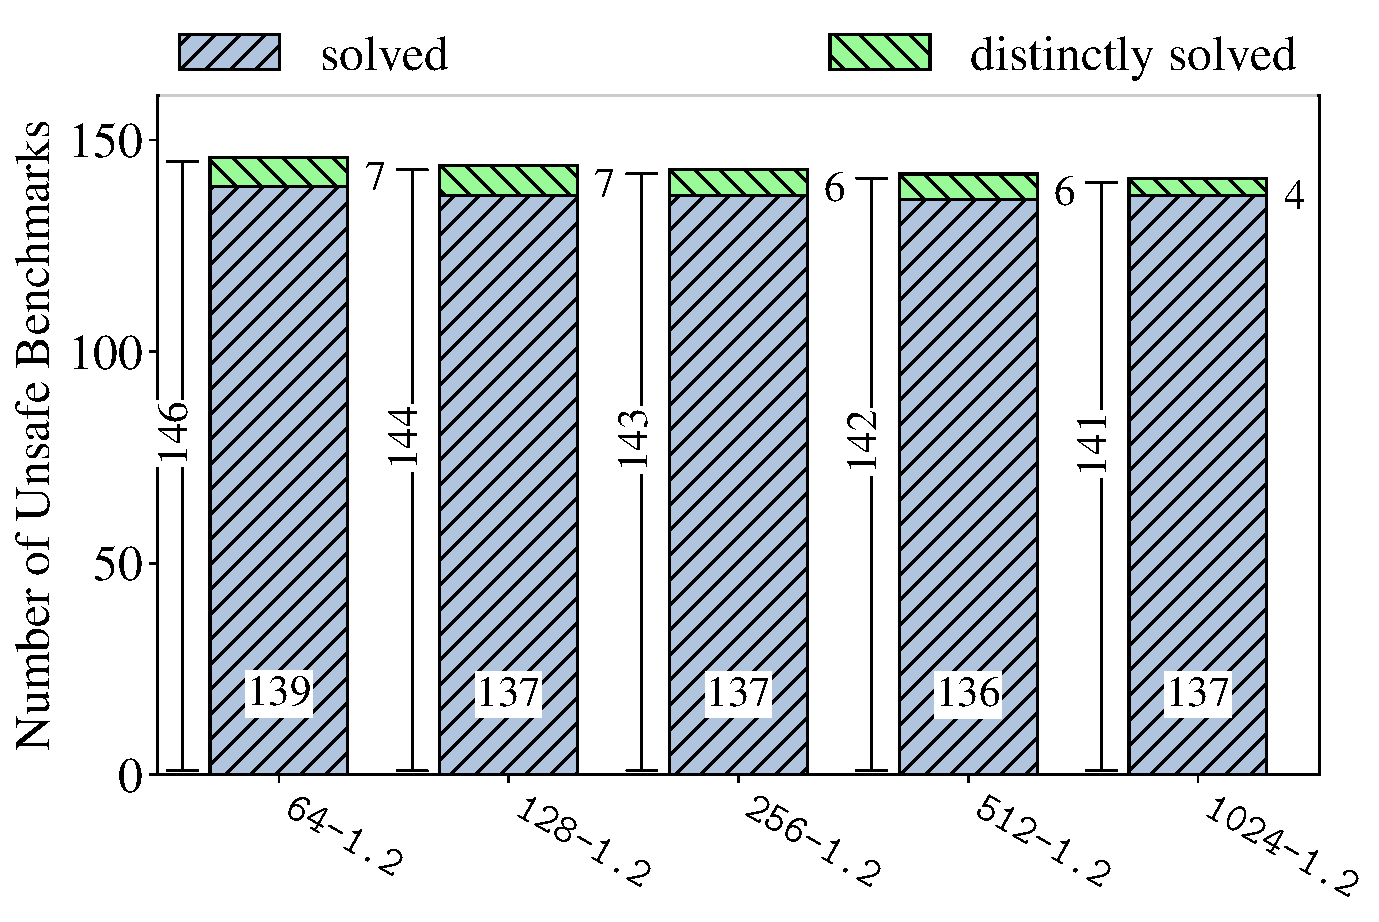
\includegraphics[width=0.49\linewidth]{images/1.2.pdf} \label{fig:car:1.2}
}
\subfigure[The overall performance of CAR and BMC.] { \label{fig:c} 
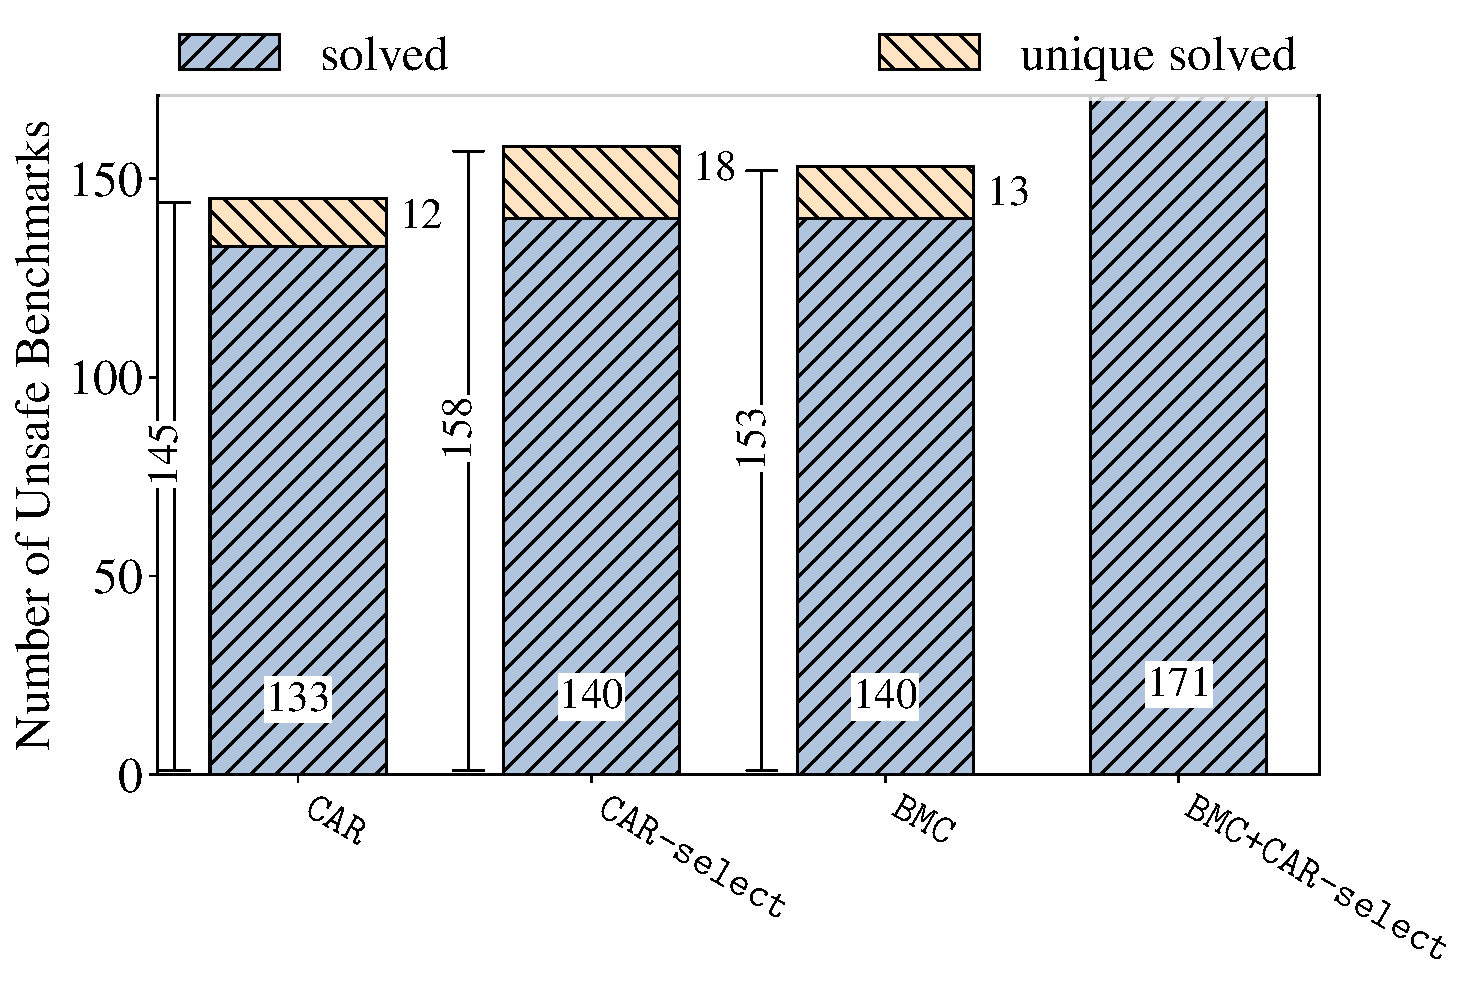
\includegraphics[width=0.49\linewidth]{images/car-bmc.pdf} \label{fig:compare}
}
\caption{Number of unsafe benchmarks solved from the experiments. The category ``distinctly solved'' benchmarks are solved by CAR with the corresponding restart policy but not by the original CAR. The ``solved'' benchmarks solved by CAR with and without the restart policy. X-axis 128-1.0 means the initial $threshold=128$, $gr=1.0$ and the same applies to others.}\label{fig:car}
\end{figure*}
\subsection{Experimental Setup}
We implement the restart policy to the SimpleCAR model checker \cite{simplecar}. As mentioned before, the restart frequency has a significant influence on the effectiveness of the restart policy. In our conjecture, the frequent restarts in CAR may not preserve the advantages already achieved, while a low frequency cannot help solve new instances. In our proposed algorithm, two parameters $threshold$ and $gr$ are introduced to determine the restart frequency in a dynamic way. We evaluate different combinations of these two parameters. We assign a relatively small value to $threshold$ and a value equal to or greater than 1 to $gr$, e.g., $threshold = 128, gr = 1.2$, aiming to avoid the disadvantage of frequent restarts by gradually increasing the threshold after each restart. 

We compare our results to those from the original CAR implemented in SimpleCAR, as well as those from BMC that is integrated in ABC tool \cite{BM10}, which is a prestigious model checker in the community and won the hardware model checking competition several times. Notably, there are kinds of BMC implementations in ABC, and we select the one invoked by the \emph{bmc2} command in the tool, which has the best performance based on previous evaluations \cite{LDPRV18}. Both SimpleCAR and ABC use the Minisat SAT solver \cite{minisat,ES04} as the computation engine for model checking. 

All the experiments are performed on a cluster which consists of 2304 processor cores in 192 nodes and each node runs RedHat 6.0 with a 2.83GHz CPU and 48GB of memory (RAM). In the experiments, the time and memory limits of each instance are set to be one hour and 8GB.
We evaluate all algorithms against 749 industrial benchmarks from the single safety property track (SINGLE) of the HWMCC in 2015 \cite{hwmcc15} and 2017 \cite{hwmcc17}. Each instance in the benchmark is an aiger model, which formalizes the And-Invertor Graph  of a circuit together with the safety property to be verified \cite{aiger}. 

This paper focuses on unsafety checking, under which a counterexample can be provided to help identify the property violation. We use the \emph{aigsim} tool from the Aiger package \cite{aigertools} to check whether the produced counterexamples are correct. We report that the counterexamples generated from all checkers pass the tests successfully.

\subsection{Results}

\subsubsection{Comparison to original CAR}
In the experiments, the original CAR is able to solve 145 unsafe instances by providing counterexamples.
To evaluate the performance of the restart policy on CAR, we first fix the initial $threshold$ to be $128$ and make the growth rate $gr$ vary from 1.0 to 16.0. The number of solved and \emph{distinctively solved} (The meaning see the figure.) instances with the corresponding parameters are shown in Fig. \ref{fig:car:128}. From the figure, the restart policy effectively expands the algorithm's diversity to find considerable new counterexamples with different configurations. In particular, the restart strategy has better results when the value of $gr$ is in $[1, 2]$, which acquires the most amount of new instances (7 or 8). Although the overall performance when $gr>2$ is similar to those when $1<gr<2$, the new instances solved with $gr>2$ can also be solved with $1<gr<2$. 


We then vary the value of $threshold$ from 64 to 1024 by fixing $gr=1.2$ (as the representative), and the corresponding results are shown in 
Fig. \ref{fig:car:1.2}. The restart policy performs the best when the value of $threshold$ is around 128, under which not only more ``distinctly solved'', but also several unique instances are detected. For example, ``oski15a08b15s'' can only be found by ``64-1.2'', ``6s351rb15'' and ``oc8051topo08''can only be solved by ``128-1.2''. In our conjecture, certain instances are sensitive to the particular combinations of the parameters that determine the frequency of restart policy. Setting the initial $threshold$ to be 1024 seems too large for an one-hour execution to make the restart strategy work. 

It should be highlighted that, although IC3/PDR can also perform differently by varying the parameters to generate the inductive clauses \cite{GR16}, it helps more significantly to prove safe instances. Meanwhile, applying the restart policy to CAR results in a better performance on solving unsafe instances, which cannot be achieved by varying different parameters inside IC3/PDR. 

\subsubsection{Comparison to BMC }
As shown in Fig. \ref{fig:compare}, the BMC implementation in ABC solve 153 unsafe instances. We combined the results of five configurations (``64-1.2'', ``128-1.2'', ``128-1.5'', ``128-3.0'' and ``256-1.2'') and the original CAR, noted as \emph{CAR-select}. Based on the results, the restart policy helps CAR find 13 more counterexamples (from 145 to 158) and 6 more unique solved (from 12 to 18) that can only be solved by CAR. Also, CAR-select solves 158 instances in total, which outperforms BMC and gains 18 instances that can not be checked by BMC. The virtual combination of CAR-select and BMC solves 171 instances, which affirms our claim that the restart policy plays a non-negligible role as a part of the portfolio in hardware model checking.
